\documentclass[graphics]{beamer}

\usepackage{graphicx}
\usepackage{verbatim}
\usepackage{wrapfig}
\useoutertheme{shadow}
%\usecolortheme{orchid}
\usecolortheme{seahorse}
\usepackage{tikzsymbols}
\usepackage{textcomp}
\usepackage{parskip}

% math commands
\newcommand{\be}{\begin{eqnarray}}
\newcommand{\ee}{\end{eqnarray}}
\newcommand{\beq}{\begin{equation}}
\newcommand{\eeq}{\end{equation}}
\def\simless{\mathbin{\lower 3pt\hbox
      {$\rlap{\raise 5pt\hbox{$\char'074$}}\mathchar"7218$}}}
\def\simgreat{\mathbin{\lower 3pt\hbox
      {$\rlap{\raise 5pt\hbox{$\char'076$}}\mathchar"7218$}}} %> or of order

% variables

\def\toonscale{0.45}
\def\mboxy#1{\mbox{\small #1}}


\begin{comment}
\AtBeginSection[]{
  \frame{
    \frametitle{Outline}
    \tableofcontents[currentsection]
  }
}
\end{comment}

\title{Helical (Parity Odd) Initial conditions
}
\subtitle{}
\author[U. Pen]{\textcolor{green}{Ue-Li Pen, ASIAA, CITA}
\\[8mm] 
}
\date{September 5, 2022}


\begin{document}

\frame{
\begin{picture}(320,250)
\put(-50,-130){
\includegraphics[width=5.5in]{Figures/delta_nu_sim.pdf}}
\end{picture}
\vspace{-3in}
\titlepage
}

%\section*{Introduction}
\section{Helicity: probe of the early universe}

\begin{comment}
  \subsection{Outline}

  \frame{
    \frametitle{Outline}
    \tableofcontents
  }
\end{comment}

   \frame{
    \frametitle{Helicity}
    \begin{itemize}
        \item Macroscopic physics (gravity, E-M, etc) are parity symmetric
        \item any observed parity asymmetry likely due to intial conditions
        \item recent claims of detection (Hou+22, )
        \item large, abstract space of parity odd configurations in
          4PCF, difficult to quantify look-elsewhere effect
        \item quadric estimator classification
        \item includes galaxy spin
        \item generation mechanisms
     \end{itemize}
}

  \frame{
    \frametitle{Quadratic forms}
    \begin{itemize}
        \item analogy: CMB lensing
        \item deflection estimator: $d_i=T \partial_i T^+$ (Okomoto-Hu)
        \item shear estimator $\Gamma_{ij}=\partial_i T\partial_j T$ (Zhu-Pen)
        \item 2 scalar, 1 pseudo scalar degree of freedom
        \item lensing power is a 4PCF, directly constrains $g_{NL}$
        \item squeezed limit $L\ll l$ reduces 4PCF to E and B lensing
          power of $L$
        \item B power is parity-odd, not helical
     \end{itemize}
}
\frame{
    \frametitle{CMB}
\vspace{-0.15in}
\hspace{-0in}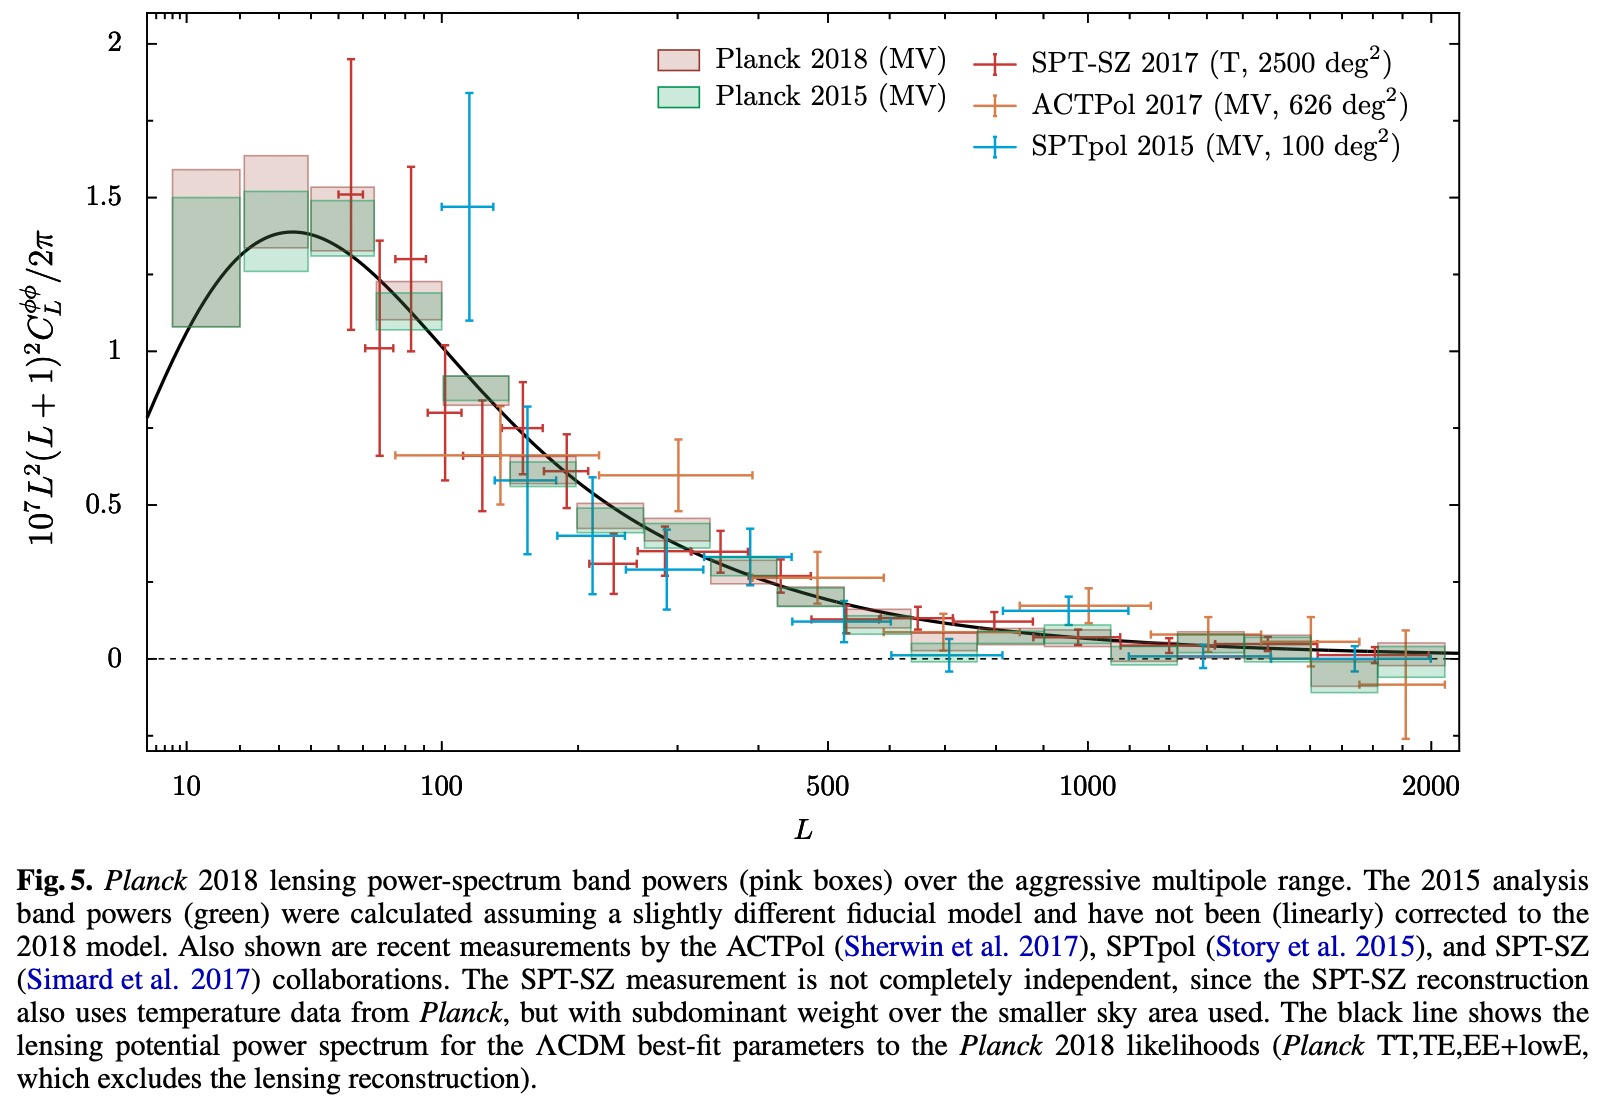
\includegraphics[width=4.2in]{Figures/plancklens.png}  

Planck 2018
  }

\frame{
    \frametitle{CMB-B}
\vspace{-0.15in}
\hspace{-0in}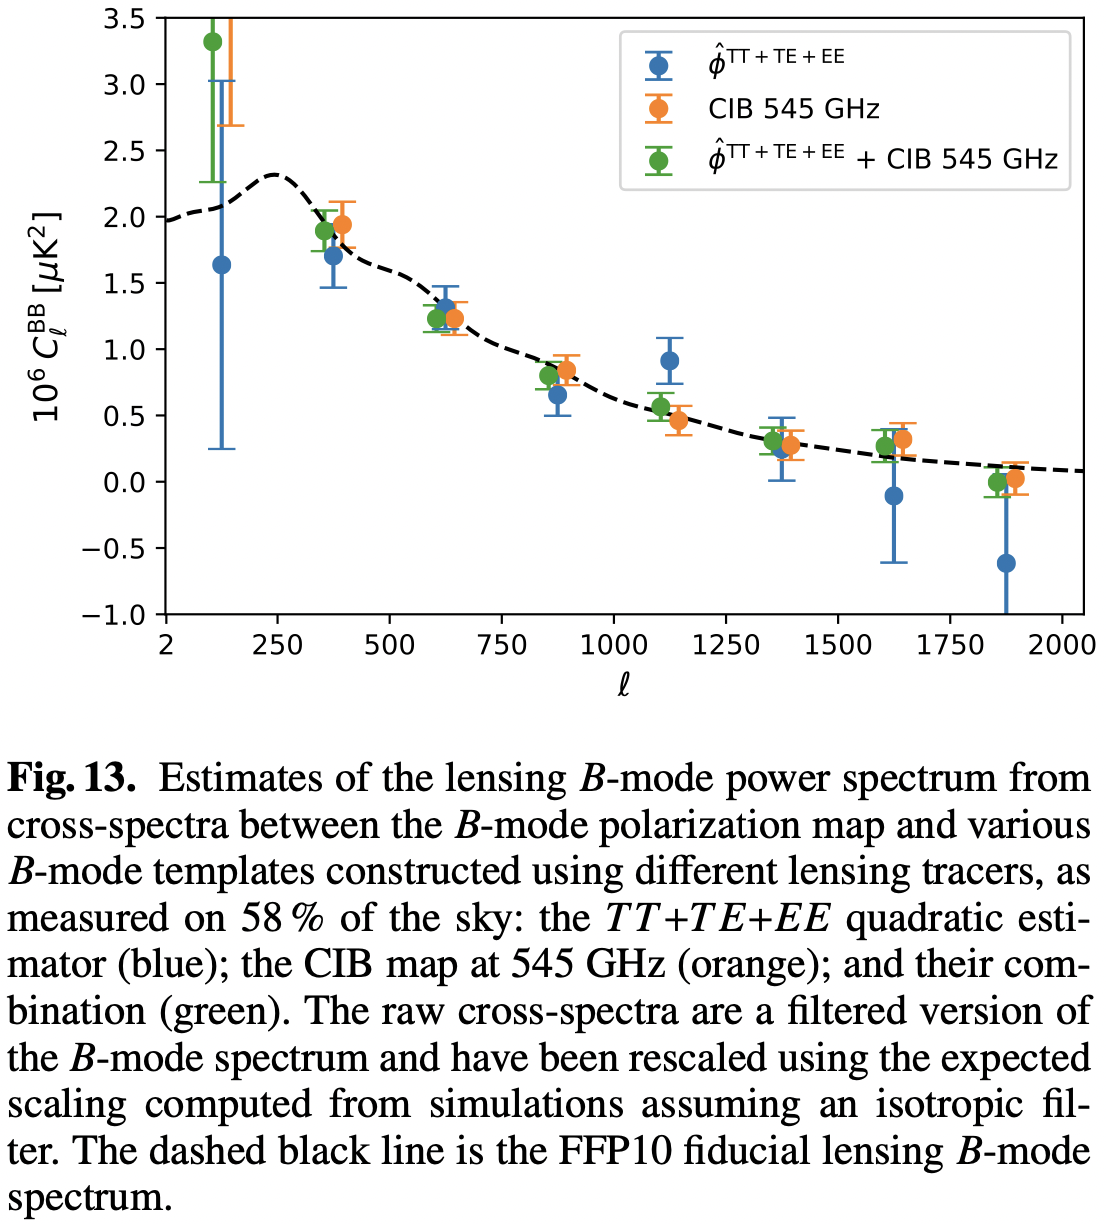
\includegraphics[width=2.8in]{Figures/plancklensb.png}  
Planck 2018
  }

  \frame{
%\vspace{-0.5in}
    \frametitle{3D quadratic form}
    \begin{itemize}
    \item Cosmic tides (ULP++2012, Masui++2010,Jeong++2012 )
    \item estimator $T_{ij}=\partial_i \bar{\delta} \partial_j
      \bar{\delta}$
    \item $T$ decomposed into 2 scalar, 2 vector, 2 tensor components
    \item scalar trace $t=T_{ii}$, longitudinal $l=\hat{k}_i\hat{k}_j (T-t\delta_{ij}/3)$
    \item vector and tensor projected onto left and right pseudoscalars
    \item $v^{L,R}=e^{L,R}_i \partial_j T_{ij}$
    \item $h^{L,R}=e^{L,R}_i e^{L,r}_j T_{ij}$
    \item helical projection operator $e^{L,R}$: eigenvectors of curl operator
    \item Helical power asymmetry: $f_H=(P_L-P_R)/(P_L+P_R)$
    \item no analogy in CMB, requires 2 parity odd (helical) d.o.f
    \item 
    \end{itemize}
    }
      

  \frame{
%\vspace{-0.5in}
    \frametitle{Helical sources}
    \begin{itemize}
    \item helical tensor modes (Jeong+12, Masui+17)
    \item Axion modes
    \item Lagrangian term $g\theta F \tilde{F}$
    \item modifies Maxwell equation $\dot{B}=\curl E+\dot{\theta}\curl B$
    \item for coherent misalignment, leads to instability in single B
      helical mode
    \item proposed for early magnetogenesis (Campanelli++05)
    \item dark sector could lead to isocurvature scalar helicity conversion
    \end{itemize}
    }
      
  \frame{
%\vspace{-0.5in}
    \frametitle{Observables}
    \begin{itemize}
    \item 4PCF -- not useful due to large dimension, difficult to
      compute covariance (8PCF!)
    \item Tidal
    \item galaxy spin
    \item magnetic field helicity
    \item 
    \item 
    \end{itemize}
    }
       
  \frame{
%\vspace{-0.5in}
    \frametitle{Helicity kinematics}
    \begin{itemize}
    \item helical vector generically sources tensor quadratic
      helicity
    \item quadratic vector helicity generation still open question
    \item 
    \item      
    \item 
    \item 
    \end{itemize}
    }
 
  \frame{
    \frametitle{Gas-DM simulations}
    \vspace{-0.1in}
    \center{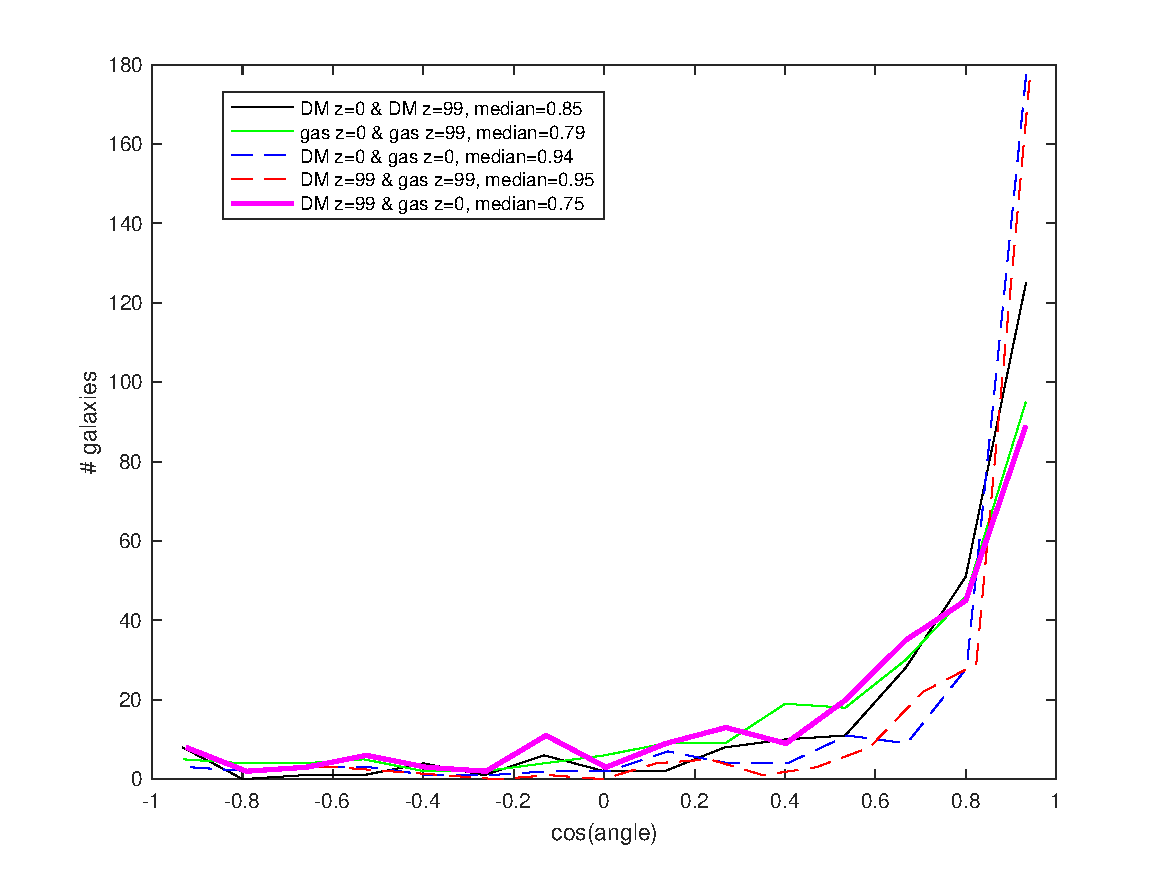
\includegraphics[width=4.01in]{Figures/Illustris_Lagrangian_AM_cosangle_distributions_allgas.pdf}}
    { Shy Genel, Illustris, private communication}
}


\frame{
    \frametitle{Measurement}
%\vspace{-0.5in}
\hspace{-0in}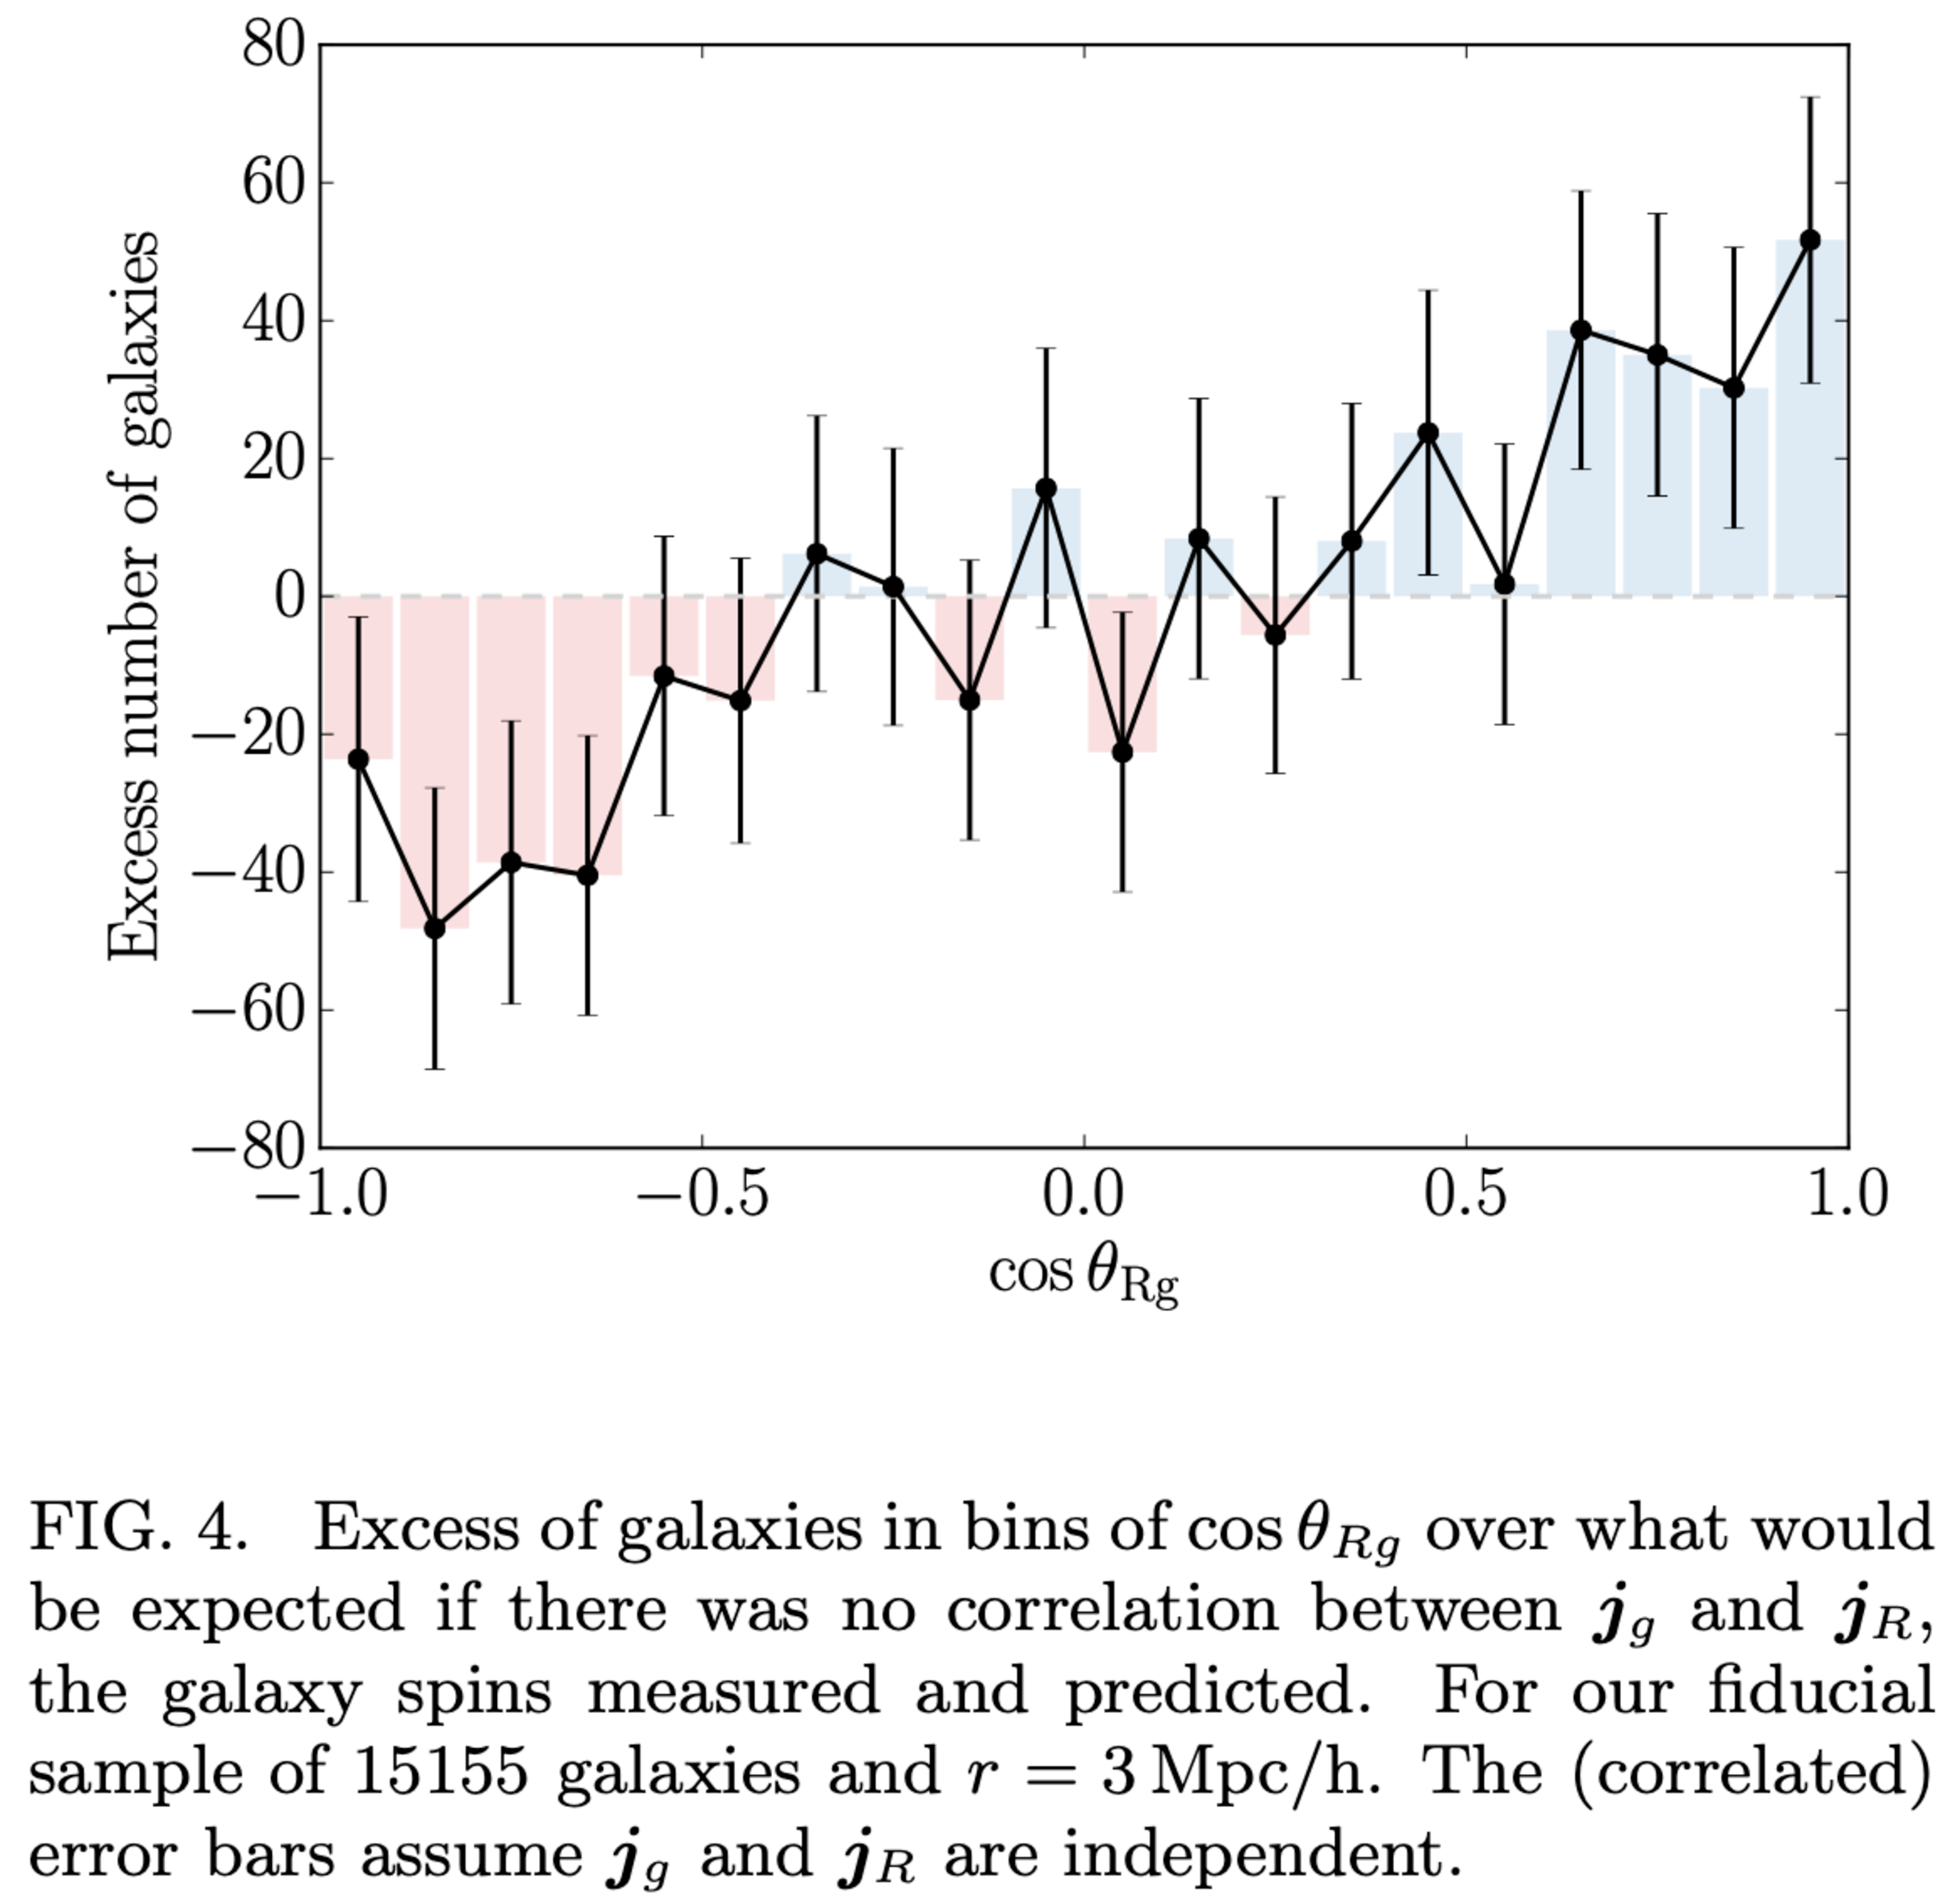
\includegraphics[width=2.9in]{Figures/spincorr.pdf}  
Motloch+ 2021
  }

 
\frame{
    \frametitle{3-D: E-mode Lagrangian}
%\vspace{-0.5in}
\hspace{-0.2in}\includegraphics[width=2.1in]{Figures/nonlinear.png}  
\vspace{0.15in}\includegraphics[width=2.1in]{Figures/reconstructed.png}  

Eulerian (L) vs Lagrangian (R) (from Yu et al 2016, 1610.7112)
  }
 
  \frame{
    \frametitle{E-mode Coordinate}
      reduce 3-D Lagrangian map to 1-D potential ({\it max Zeldovich}):
    \begin{eqnarray}      
{\rm potential\ deformation\ \ \ \ \ }  x^i &=& \xi^\mu \delta^i_\mu + \frac{\partial \phi}{\partial
    \xi^\mu}\delta^{i\mu}\nonumber\\
{\rm dreibein\ \ \ \ \ \  } e^i_\mu &\equiv& \partial x^i / \partial \xi ^ \mu \nonumber\\
 {\rm volume\  element\ \ \ \ }\sqrt{g} &\equiv& \mathrm{det}\left| e^i_\mu\right|\nonumber\\
{\rm mass\ coordinate \ \ \ \ \ }    \rho \sqrt{g}&=&\mathrm{Const.}\nonumber\\
    \partial _\mu (\rho \sqrt{g} e^\mu _i \delta^{i\nu}
    \partial_\nu \dot{\phi})&=&\langle\rho\rangle-\rho \sqrt{g}
\label{eqn:dif}
\end{eqnarray}
Solve Monge-Amp\'ere eqn (\ref{eqn:dif}) using multigrid (Pen 1995):
unique bijective mass coordinate.  See also Tully/Peebles, Mohayaee+, Goldberg, Schmidtfull, Wang+, Seljak,
Zaldarriaga, Hada/Eisenstein, Shi/Brikin/Li+, Jasche+, Sarpa+
}

 \frame{
    \frametitle{Predicting Neutrino Torques}
    \begin{itemize}
      \item $\nu$ gravitational field (large scale tide) torques CDM (small scale inertia)
      \item $\Delta x (q) = q^j \partial_i\partial_j \psi$
        \item $I_c \sim T_c$: both describe particle displacement
        \item $j_\nu = \epsilon I_c T_\nu \sim  \epsilon T_c T_\nu$
        \item Neutrino tidal torque is predictable observable from
          displacement potential
     \end{itemize}
 }
 
  \frame{
    \frametitle{Movie}
    {\tt http://cita.utoronto.ca/\~\,haoran/thnu/movie.html}
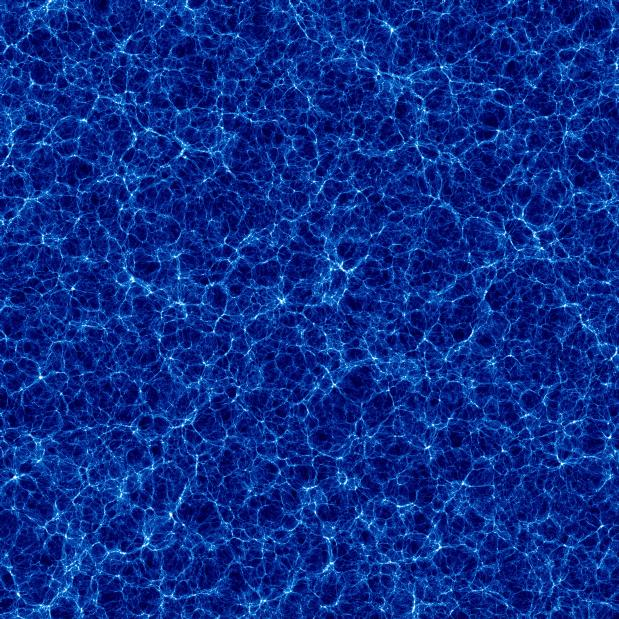
\includegraphics[width=4.2in]{Figures/thnucdmlowres.jpg}
}

  \frame{
    \frametitle{Illustration}
\vspace{-0.5in}\hspace{-0.6in}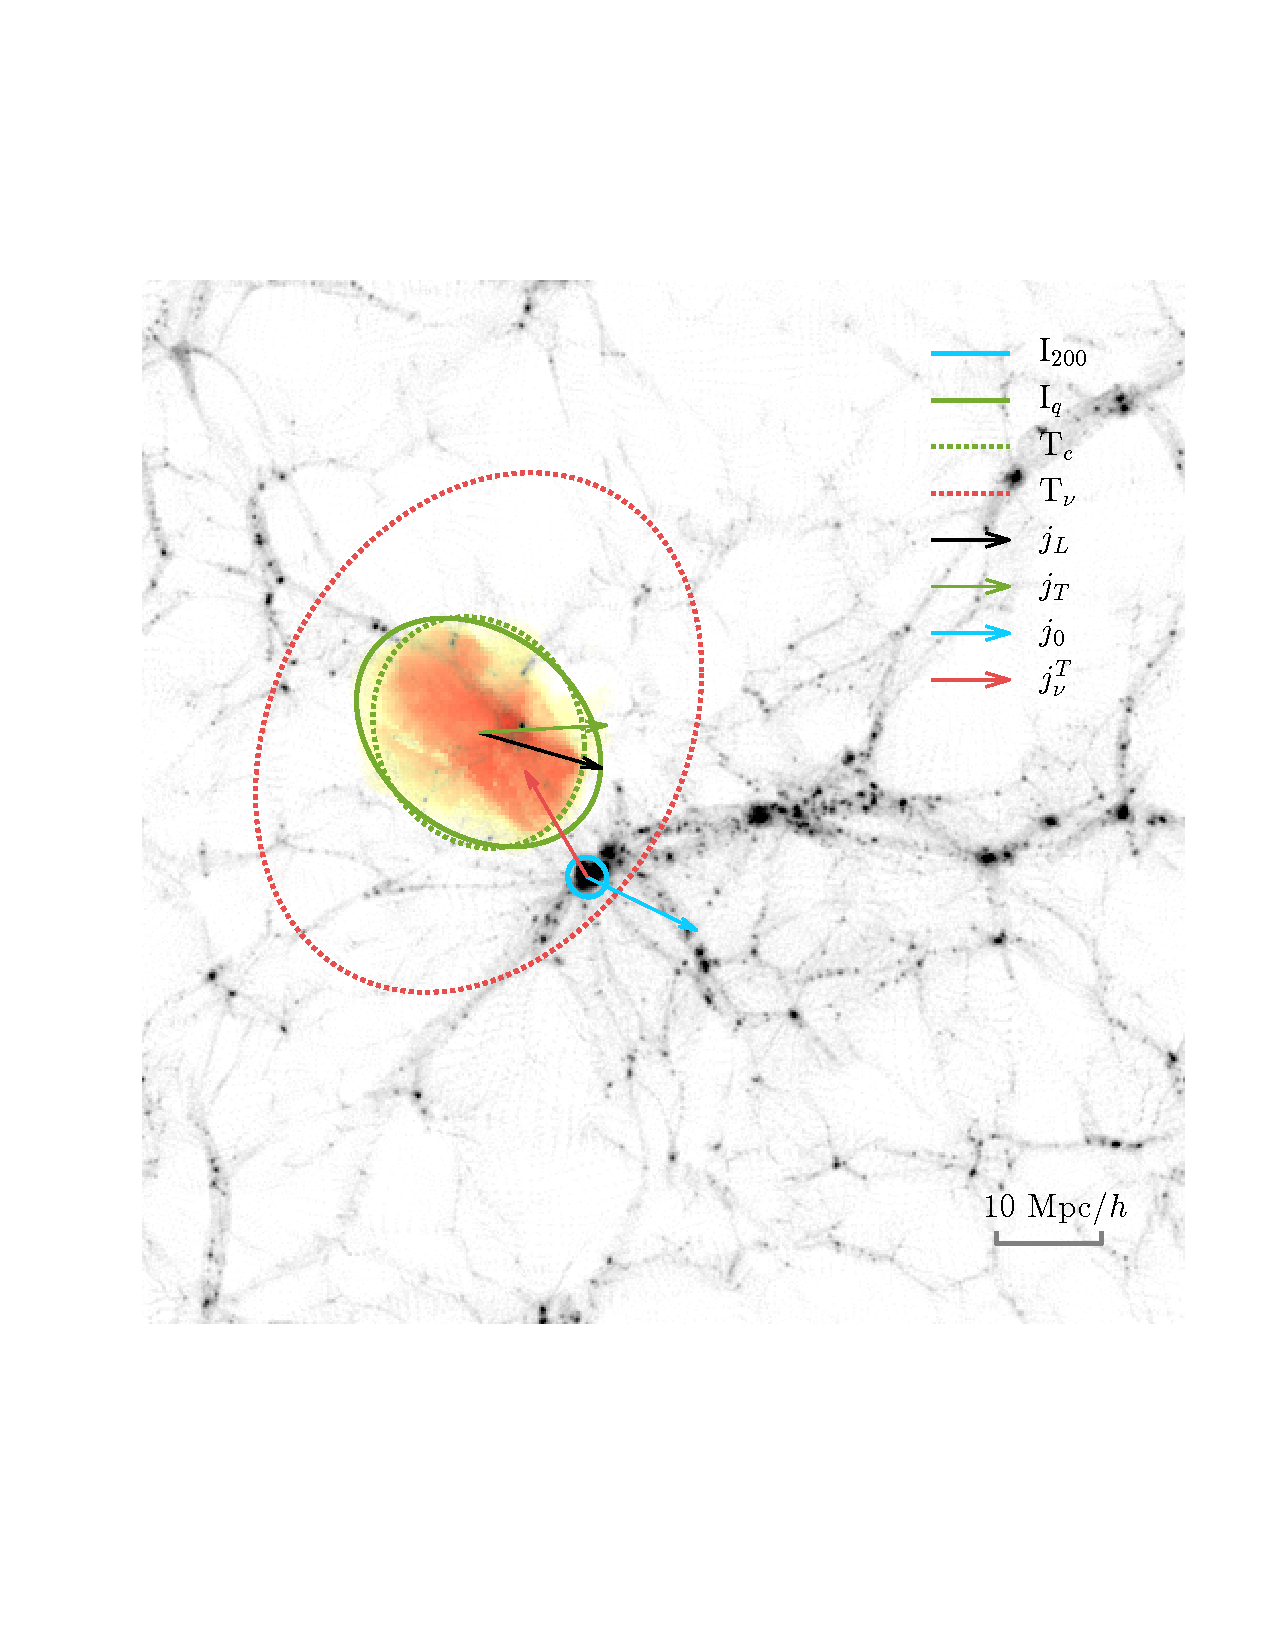
\includegraphics[width=5.0in]{Figures/f1.pdf}
}

 \frame{
    \frametitle{Size estimate}
    \begin{itemize}
    \item $|j_\nu/j_c| \sim 10^{-4} (f_\nu /0.003) [\sqrt{P(k_{\rm FS})/P(k_{\rm vir})}/0.03]$
    \item agrees with simulation measurement
    \item need $n> 10^8$ galaxy spins
    \item accessible in next generation 21cm surveys
     \end{itemize}
  }


  
\frame{
\vspace{-0.5in}
    \frametitle{Helicity}
    \begin{itemize}
    \item statistical isotropy and homogeneity allows for helicity asymmetry (e.g. weak force)
        \item NOT Goedel/Longo effect (``net $k$ independent left/right spin'')
        \item angular momentum measures twist of tidal tensor
        \item helicity measures twist projected along $k$ vector 
     \end{itemize}
  }

  \frame{
    \frametitle{Nature}
\vspace{-0.3in}\center{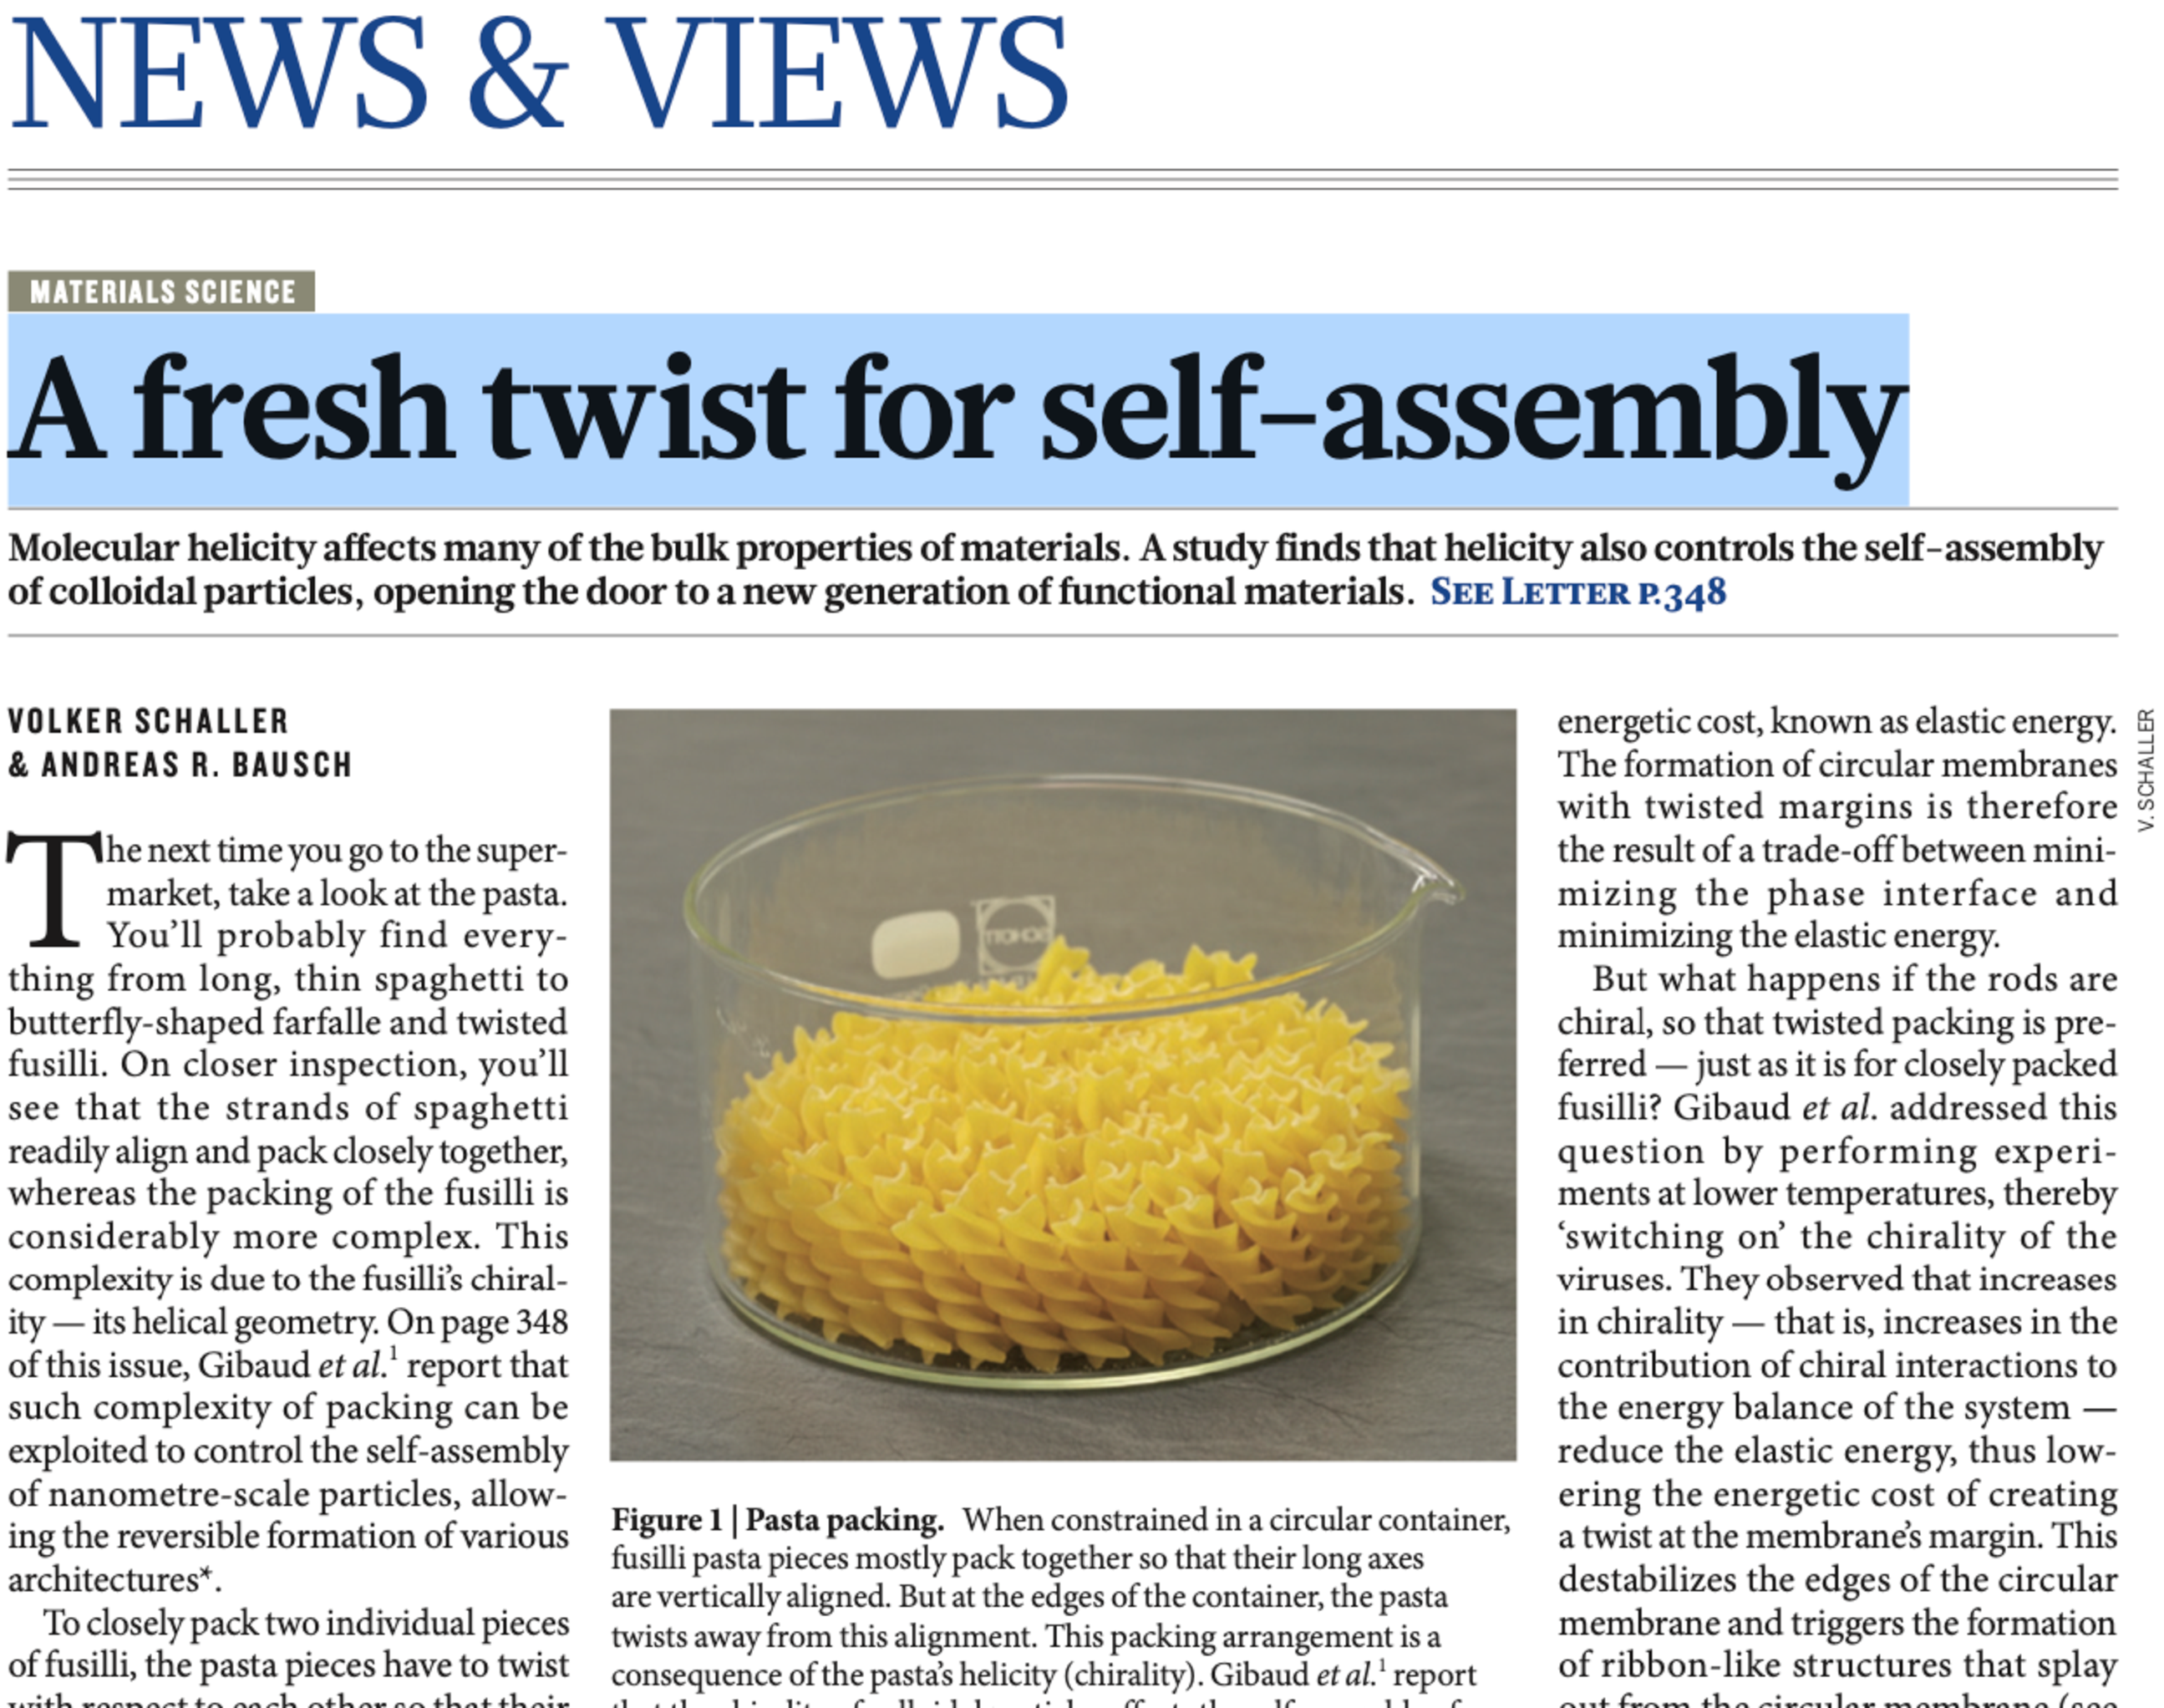
\includegraphics[width=4.0in]{Figures/twist.pdf}}
V Schaller \& A. Bausch, Nature, 481, 268
}
  \frame{
    \frametitle{Pastarimeter}
    %\vspace{-0.3in}
    \center{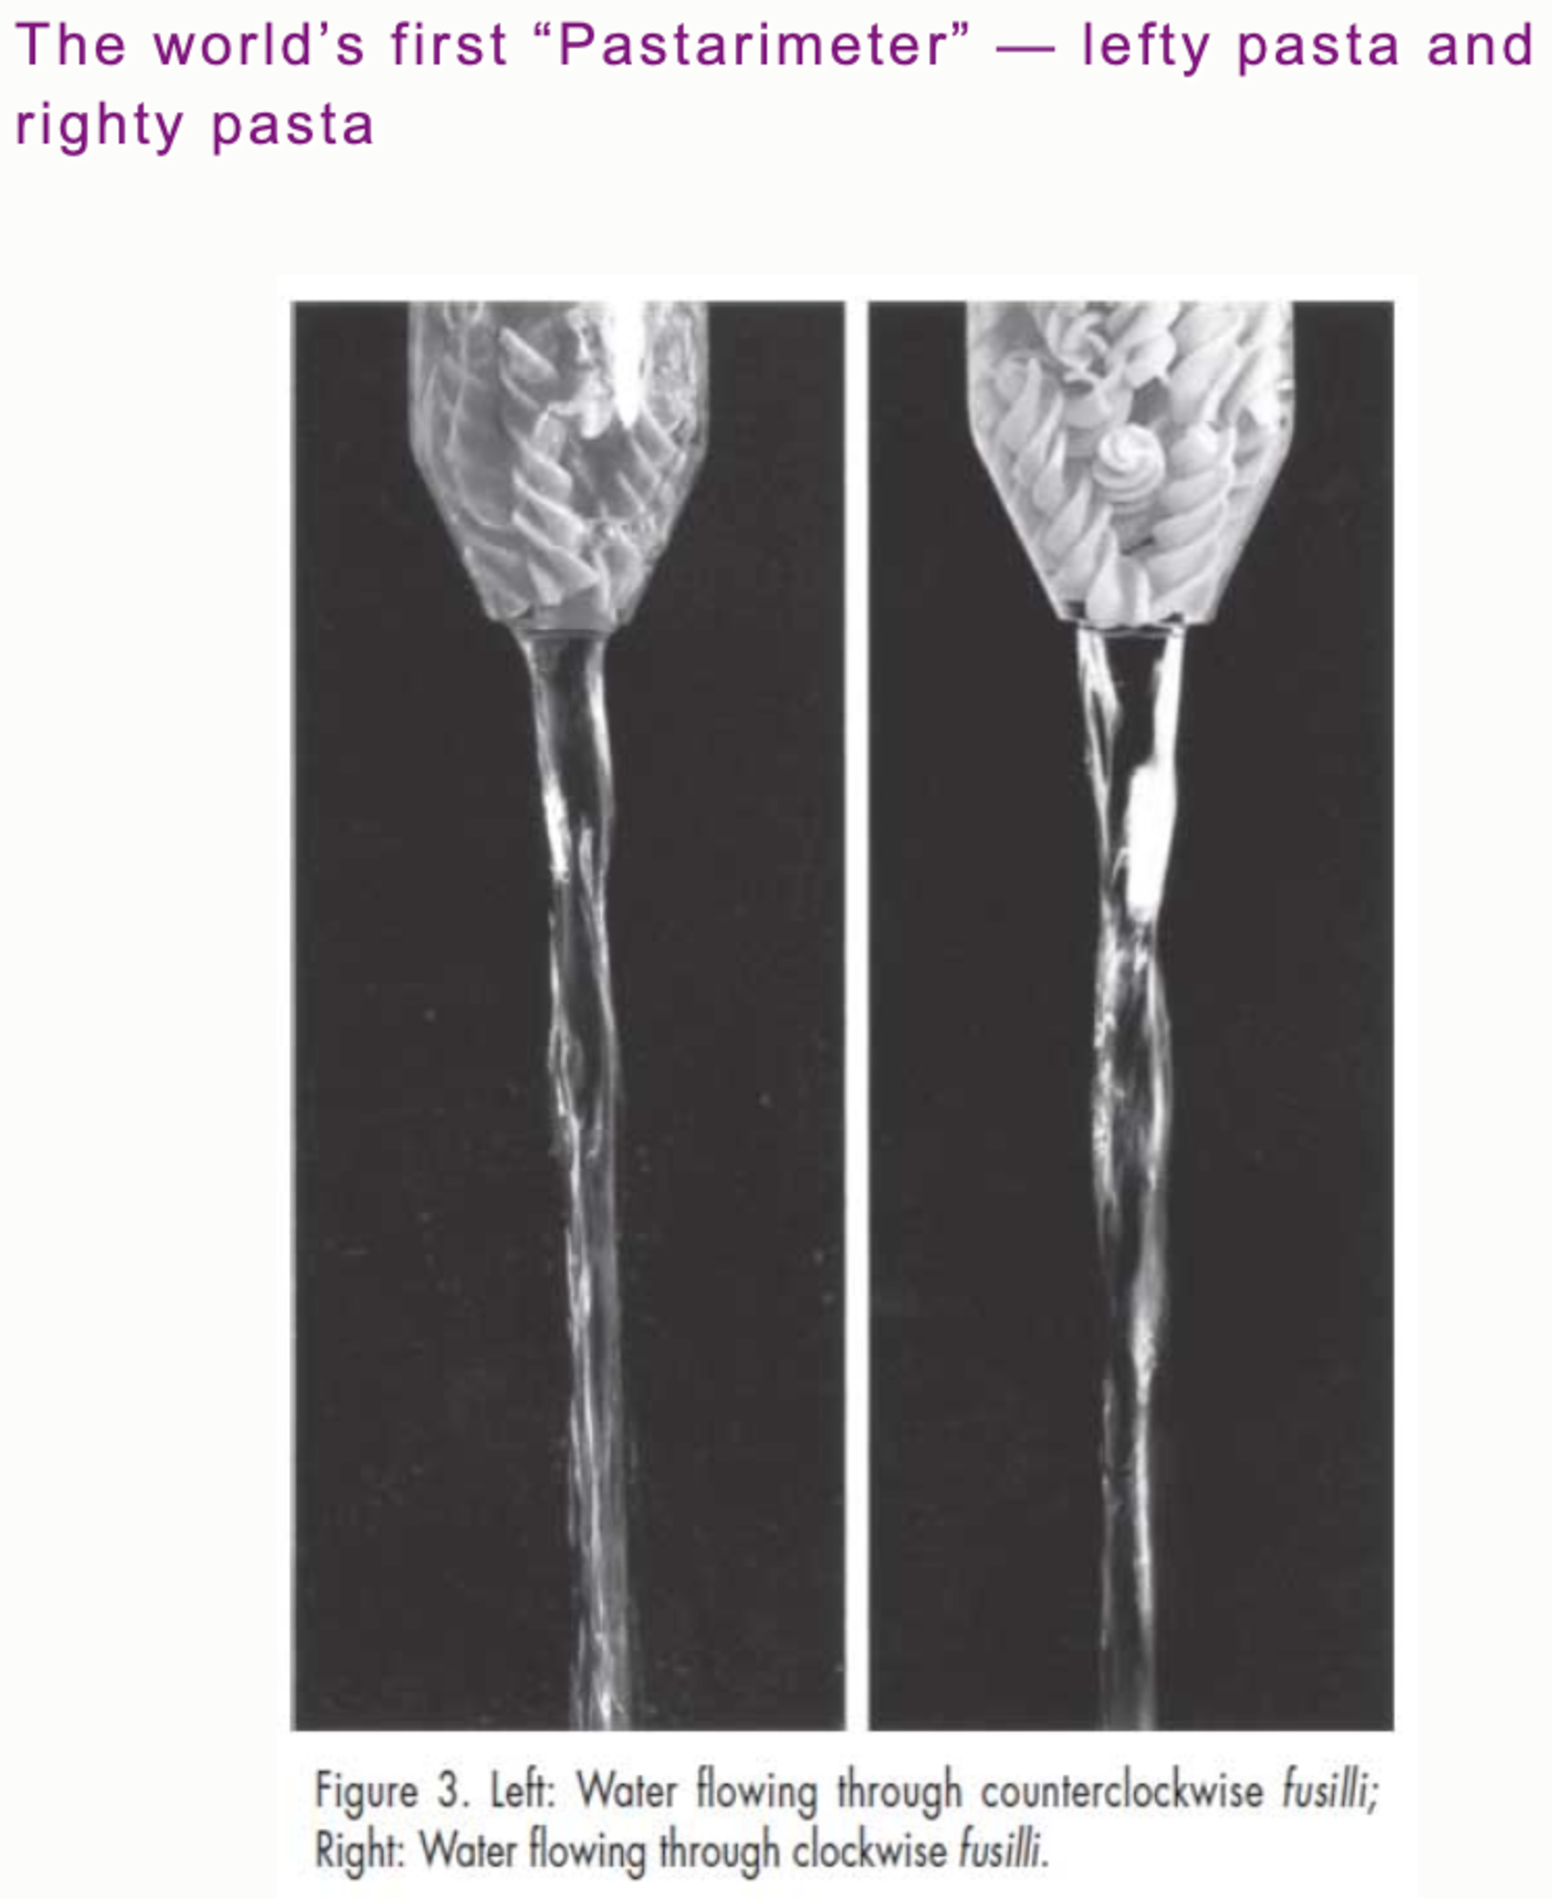
\includegraphics[width=2.5in]{Figures/pastarimeter.pdf}}
{\tiny Saxon et al 2002, J. Chem. Ed, 79, 1214}
}


 \frame{
    \frametitle{ELUCID projection}
    \begin{itemize}
    \item $J^\mathrm{IC}_a=  \epsilon_{abc}
\partial_{bk} \phi^r
\partial_{kc} \rho^r$
    \item  $\mathbb{P}^{L/R}_{ab}(\mathbf{k}) = 
  \frac{1}{2}
  \left[
  \(\delta_{ab} - \hat k_a \hat k_b\) 
  \pm    i \epsilon_{abc} \hat k_c \right] $
    \item   $\tilde J^\mathrm{IC}_{L/R,a}(\mathbf{k}) \equiv
  \mathbb{P}^{L/R}_{ab}(\mathbf{k}) 
  \tilde J^\mathrm{IC}_b(\mathbf{k})$
    \item  $\mu_X = \left\langle 
  \frac{\bs{J}^g}{|\bs{J}^g|}
  \cdot
  \frac{\bs{J}^\mathrm{IC}_X}{|\bs{J}^\mathrm{IC}_X|}
  \right\rangle \ \ \ \ \ X \in \{L, R\}$
\item $\mu_- = \mu_L - \mu_R$
     \end{itemize}
  }


  
\frame{
\vspace{-0.5in}
    \frametitle{Helicity results}
    \begin{itemize}
    \item   $\mu_L &=& \(0.41 \pm 0.53\) \times 10^{-2}$  maximal left is allowed
      \item $\mu_R &=& \(1.99 \pm 0.53\) \times 10^{-2} $  maximal right is disfavoured!
      \item $\mu_- = \(-1.58 \pm 0.75\) \times 10^{-2}$  Parity symmetry is allowed \dSmiley % \DejaSans{ ☺}
     \end{itemize}
  }

\frame{
\vspace{-0.5in}
    \frametitle{Helicity IC}
    \begin{itemize}
    \item  Helicity is probe of primordial non-gaussianity 4 point function (e.g. Cahn+ 2021)
    \item constructable in N-body initial conditions
    \item maximal violation straightforward to implement numerically, consistent with observations
    \item  potentially related to inflationary two field chiral coupling 
     \end{itemize}
  }

  
\frame{
\vspace{-0.5in}
    \frametitle{Conclusions}
    \begin{itemize}
      \item galaxy spins: new probe of initial conditions
      \item predictable from observable displacement field using
        non-linear reconstruction
      \item computationally straightforward, mass coordinate
            similar to Lagrangian
          \item already observable, scalable to much larger surveys
          \item parity odd field, less likely to be contaminated
          \item unique probes of neutrinos, helicities, etc...
     \end{itemize}
  }


\end{document}
